\documentclass{article}
\usepackage[margin=2.5cm, a4paper]{geometry}
\usepackage{amsmath}
\usepackage{tikz}
\usetikzlibrary{arrows.meta, calc}
\usepackage{xcolor}
\usepackage{caption}

% ── colour palette ────────────────────────────────────────────────────────────
\definecolor{desblue}   {RGB}{31,119,180}   % DES elevation line
\definecolor{gosplred}  {RGB}{200, 40, 40}  % GoSPL call markers
\definecolor{extrapgrn} {RGB}{ 44,160, 44}  % extrapolated / new-rate elements
\definecolor{limitorg}  {RGB}{220,120,  0}  % limiter line
\definecolor{shadegray} {RGB}{225,225,225}  % "skipped steps" background

% ── shared style macros ───────────────────────────────────────────────────────
\tikzset{
  axis/.style      = {->, thick},
  gospl line/.style= {gosplred, dashed, thick},
  des line/.style  = {desblue,  very thick},
  extrap line/.style = {extrapgrn, very thick, dashed},
  rate dot/.style  = {extrapgrn, circle, inner sep=0pt, minimum size=6pt, fill},
  known dot/.style = {desblue,  circle, inner sep=0pt, minimum size=8pt, fill},
  annotation/.style= {font=\scriptsize, ->, thick},
}

\begin{document}

% ══════════════════════════════════════════════════════════════════════════════
%  FIGURE 1 — Old lump-sum vs. new gradual application
% ══════════════════════════════════════════════════════════════════════════════
\begin{figure}[h]
\centering
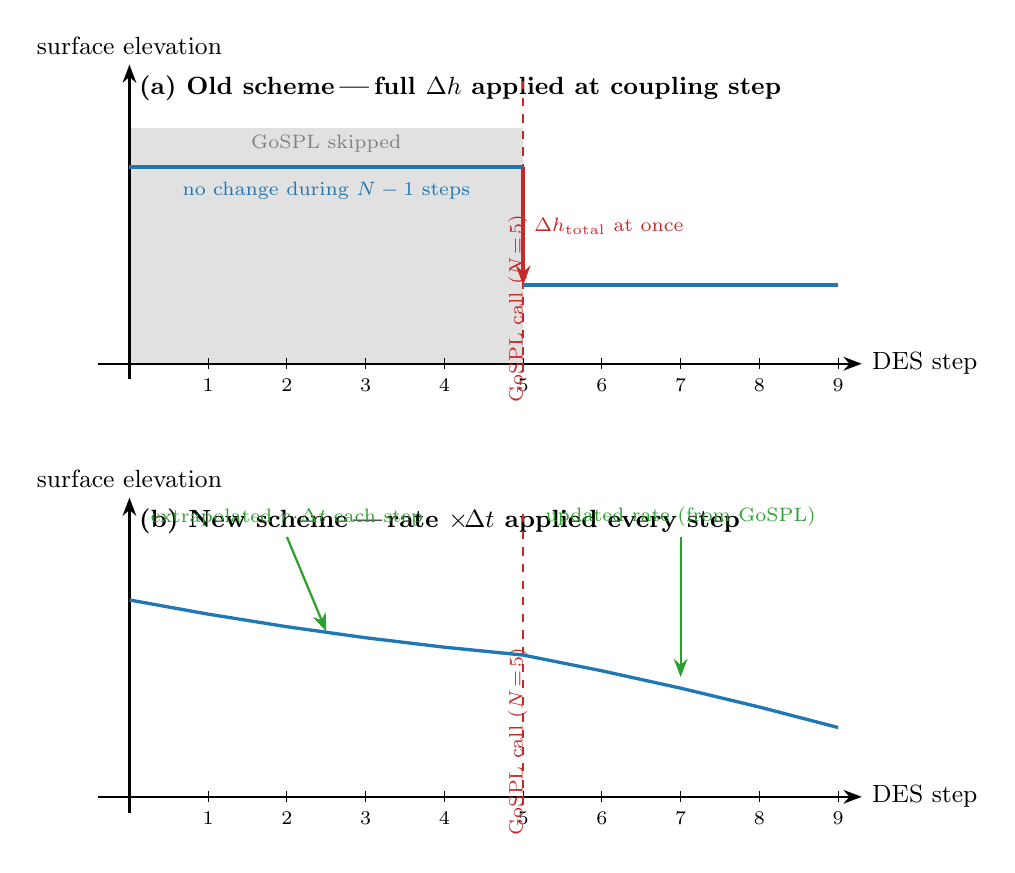
\begin{tikzpicture}[>=Stealth, font=\small, x=1cm, y=1cm]

  % ── (a) OLD ────────────────────────────────────────────────────────────────
  \begin{scope}[yshift=0cm]

    \node[anchor=west, font=\bfseries\small] at (0.7, 3.7)
      {(a)~Old scheme\,—\,full $\Delta h$ applied at coupling step};

    % shaded "waiting" region (steps 0–5 where GoSPL is skipped)
    \fill[shadegray] (0.7, 0.2) rectangle (5.7, 3.2);
    \node[gray, font=\scriptsize] at (3.2, 3.0) {GoSPL skipped};

    % axes
    \draw[axis] (0.3, 0.2) -- (10.0, 0.2) node[right] {DES step};
    \draw[axis] (0.7, 0.0) -- (0.7, 4.0)  node[above] {surface elevation};

    % x-axis ticks
    \foreach \i in {1,...,9}{
      \draw ({0.7+\i}, 0.27) -- ({0.7+\i}, 0.13)
        node[below, font=\scriptsize] {\i};
    }

    % GoSPL call marker at step 5
    \draw[gospl line] (5.7, 0.1) -- (5.7, 3.8);
    \node[gosplred, rotate=90, anchor=south, font=\scriptsize]
      at (5.88, 0.9) {GoSPL call ($N\!=\!5$)};

    % elevation line: flat → sudden drop → flat
    \draw[des line] (0.7, 2.7) -- (5.7, 2.7);
    \draw[gosplred, very thick, -{Stealth[length=7pt]}]
      (5.7, 2.7) -- (5.7, 1.2)
      node[midway, right, gosplred, font=\scriptsize]
        {$\Delta h_{\mathrm{total}}$ at once};
    \draw[des line] (5.7, 1.2) -- (9.7, 1.2);

    % annotation
    \node[desblue, font=\scriptsize] at (3.2, 2.4)
      {no change during $N-1$ steps};

  \end{scope}

  % ── (b) NEW ────────────────────────────────────────────────────────────────
  \begin{scope}[yshift=-5.5cm]

    \node[anchor=west, font=\bfseries\small] at (0.7, 3.7)
      {(b)~New scheme\,—\,rate $\times\!\Delta t$ applied every step};

    % axes
    \draw[axis] (0.3, 0.2) -- (10.0, 0.2) node[right] {DES step};
    \draw[axis] (0.7, 0.0) -- (0.7, 4.0)  node[above] {surface elevation};

    % x-axis ticks
    \foreach \i in {1,...,9}{
      \draw ({0.7+\i}, 0.27) -- ({0.7+\i}, 0.13)
        node[below, font=\scriptsize] {\i};
    }

    % GoSPL call marker at step 5
    \draw[gospl line] (5.7, 0.1) -- (5.7, 3.8);
    \node[gosplred, rotate=90, anchor=south, font=\scriptsize]
      at (5.88, 0.9) {GoSPL call ($N\!=\!5$)};

    % elevation interval 1 (steps 0–5): gradual with slight extrapolation
    % (rate accelerates slightly as the trend from prev→pending is projected)
    \draw[des line]
      (0.7, 2.7) -- (1.7, 2.52) -- (2.7, 2.36)
                 -- (3.7, 2.22) -- (4.7, 2.10) -- (5.7, 2.00);

    % elevation interval 2 (steps 5–9): new, slightly steeper rate
    \draw[des line]
      (5.7, 2.00) -- (6.7, 1.80) -- (7.7, 1.58) -- (8.7, 1.34) -- (9.7, 1.08);

    % annotations
    \draw[extrapgrn, annotation]
      (2.7, 3.5) node[extrapgrn, anchor=south, font=\scriptsize]
        {extrapolated $r\!\cdot\!\Delta t$ each step}
      -- (3.2, 2.30);

    \draw[extrapgrn, annotation]
      (7.7, 3.5) node[extrapgrn, anchor=south, font=\scriptsize]
        {updated rate (from GoSPL)}
      -- (7.7, 1.72);

  \end{scope}

\end{tikzpicture}
\caption{Comparison of the old and new coupling schemes for $N=5$ steps between GoSPL calls.
  \textbf{(a)}~Old scheme: the full elevation change $\Delta h$ is applied as a lump sum
  at the coupling step, creating an impulsive perturbation.
  \textbf{(b)}~New scheme: the erosion rate computed at each GoSPL call is applied
  gradually to every DES step in the following interval, using linear extrapolation
  to project how the rate is evolving.}
\end{figure}

\clearpage

% ══════════════════════════════════════════════════════════════════════════════
%  FIGURE 2 — Linear rate extrapolation detail
% ══════════════════════════════════════════════════════════════════════════════
\begin{figure}[h]
\centering
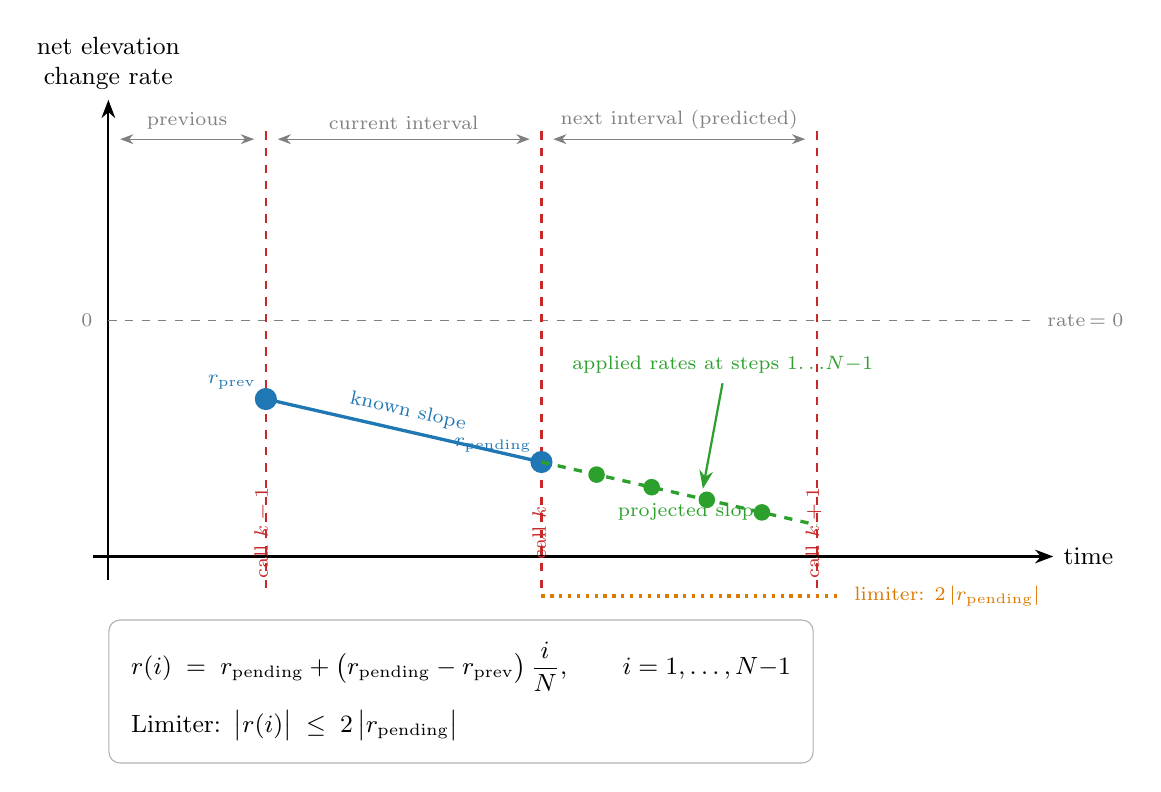
\begin{tikzpicture}[>=Stealth, font=\small, x=1cm, y=1cm]

  % axes  (y is plotted inverted: more erosion = further down)
  \draw[axis] (-0.2, 0) -- (12.0, 0) node[right] {time};
  \draw[axis] (0, -0.3) -- (0, 5.8)
    node[above, align=center, font=\small]
      {net elevation\\change rate};

  % zero-rate reference line
  \draw[gray, dashed] (0, 3.0) -- (11.8, 3.0)
    node[right, font=\scriptsize, gray] {rate\,$=0$};
  \node[gray, font=\scriptsize, anchor=east] at (-0.08, 3.0) {$0$};

  % ── GoSPL call markers at x = 2, 5.5, 9 ──────────────────────────────────
  \foreach \x/\lbl in {2.0/{k-1}, 5.5/{k}, 9.0/{k+1}}{
    \draw[gospl line] (\x, -0.4) -- (\x, 5.5);
    \node[gosplred, rotate=90, anchor=south, font=\scriptsize]
      at (\x+0.18, 0.3) {call $\lbl$};
  }

  % ── interval bracket labels ───────────────────────────────────────────────
  \foreach \xa/\xb/\lbl in
      {0.0/2.0/previous,
       2.0/5.5/{current interval},
       5.5/9.0/{next interval (predicted)}}{
    \draw[gray, <->] (\xa+0.15, 5.3) -- (\xb-0.15, 5.3)
      node[midway, above, font=\scriptsize, gray] {\lbl};
  }

  % ── known rate points ─────────────────────────────────────────────────────
  %  prev_rate    at (2.0, 2.0)   — small erosion (slightly below zero line)
  %  pending_rate at (5.5, 1.2)   — stronger erosion
  \coordinate (PR) at (2.0, 2.0);
  \coordinate (PE) at (5.5, 1.2);

  % known-history line (solid)
  \draw[desblue, very thick] (PR) -- (PE)
    node[midway, above, sloped, desblue, font=\scriptsize] {known slope};

  % rate dots
  \node[known dot] at (PR) {};
  \node[desblue, anchor=south east, font=\scriptsize] at (PR)
    {$r_{\mathrm{prev}}$};

  \node[known dot] at (PE) {};
  \node[desblue, anchor=south east, font=\scriptsize] at (PE)
    {$r_{\mathrm{pending}}$};

  % ── extrapolated dashed line ───────────────────────────────────────────────
  % slope = (1.2−2.0)/(5.5−2.0) = −0.8/3.5 ≈ −0.229 per x-unit
  % at x=9.0: y = 1.2 + (−0.229)×(9.0−5.5) = 1.2 − 0.8 = 0.4
  \draw[extrap line] (PE) -- (9.0, 0.4);
  \node[extrapgrn, font=\scriptsize, anchor=north] at (7.4, 0.8)
    {projected slope};

  % ── applied sub-step rates at i = 1…N−1 (N=5) ────────────────────────────
  % Interval spans x ∈ [5.5, 9.0], step spacing = 3.5/5 = 0.7
  % r(i) = 1.2 + (1.2−2.0)×i/5 = 1.2 − 0.16×i
  \foreach \i in {1,...,4}{
    \pgfmathsetmacro{\xi}{5.5 + 0.7*\i}
    \pgfmathsetmacro{\yi}{1.2 - 0.16*\i}
    \node[rate dot] at (\xi, \yi) {};
  }

  % annotation for sub-step dots
  \draw[extrapgrn, annotation]
    (7.8, 2.2) node[extrapgrn, anchor=south, font=\scriptsize]
      {applied rates at steps $1{\ldots}N{-}1$}
    -- (7.55, 0.86);

  % ── limiter line ──────────────────────────────────────────────────────────
  % |pending| = 3.0 − 1.2 = 1.8 (distance from zero line)
  % limit = 2 × 1.8 = 3.6 below zero → y = 3.0 − 3.6 = −0.6
  % draw at −0.5 (visible near bottom of axes) with annotation
  \draw[limitorg, dotted, very thick] (5.5, -0.5) -- (9.3, -0.5);
  \node[limitorg, font=\scriptsize, anchor=west] at (9.35, -0.5)
    {limiter: $2\,|r_{\mathrm{pending}}|$};

  % ── formula box ───────────────────────────────────────────────────────────
  \node[draw=gray!60, fill=white, rounded corners=4pt,
        inner sep=8pt, font=\small, align=left, anchor=north west]
    at (-0.0, -0.8) {%
      $r(i)
        \;=\; r_{\mathrm{pending}}
          + \bigl(r_{\mathrm{pending}} - r_{\mathrm{prev}}\bigr)\,
            \dfrac{i}{N},
        \qquad i = 1, \ldots, N{-}1$
      \\[6pt]
      Limiter:\enspace
        $\bigl|r(i)\bigr| \;\leq\; 2\,\bigl|r_{\mathrm{pending}}\bigr|$
  };

\end{tikzpicture}
\caption{Linear rate extrapolation across coupling intervals.
  At each GoSPL call the two most recent interval-average rates
  ($r_{\mathrm{prev}}$, $r_{\mathrm{pending}}$) define a \emph{known slope}
  (solid blue line).
  That slope is projected forward (dashed green line) to fill the
  \emph{next} coupling interval; green dots mark the rate actually applied
  at each of the $N{-}1$ non-coupling DES steps.
  A $2\times$ limiter (orange dotted line) prevents runaway extrapolation
  when rates change abruptly.}
\end{figure}

\end{document}
